\documentclass{report}
\usepackage[utf8]{inputenc}
\usepackage{amssymb}
\usepackage{amsmath}
\usepackage{hyperref}
\usepackage{tcolorbox}
\usepackage{physics}
\tcbuselibrary{theorems}

% Things I use, but too lazy to find how again

%%%%%%%%%%%%%%%%%%%%%%%%%%%%%%%%%%%%%%%%%%%%%%%%%%%%
% Make a hyperlink to another section:
% \hyperref[sec:hello]{Word of text} (set link to hello)

% \section{Hello World} 
% \label{sec:hello} (define a label for the section
%%%%%%%%%%%%%%%%%%%%%%%%%%%%%%%%%%%%%%%%%%%%%%%%%%%%
% Make an unordered list:
% \begin{itemize}
%   \item 
%   \item
% \end{itemize}
%%%%%%%%%%%%%%%%%%%%%%%%%%%%%%%%%%%%%%%%%%%%%%%%%%%%
% Make an ordered list:
% \begin{enumerate}
%   \item 
%   \item
% \end{itemize}
%%%%%%%%%%%%%%%%%%%%%%%%%%%%%%%%%%%%%%%%%%%%%%%%%%%%
% Make a matrix
%\begin{bmatrix}
%        x_1y_1 & x_1y_2 & \dots  & x_1y_m \\
%        x_2y_1 & x_2y_2 & \dots  & x_2y_m \\
%        \vdots & \vdots & \ddots & \vdots \\
%        x_ny_1 & a_{m2} & \dots  & x_ny_m \\
%   \end{bmatrix}
%%%%%%%%%%%%%%%%%%%%%%%%%%%%%%%%%%%%%%%%%%%%%%%%%%%%
% Make an equation:
% \begin{equation}
% ...
% \end{equation}
%%%%%%%%%%%%%%%%%%%%%%%%%%%%%%%%%%%%%%%%%%%%%%%%%%%%
% Theorems:
%\begin{mytheo}{Title}{NameOfTheorem}
% ...
%\end{mytheo}
%%%%%%%%%%%%%%%%%%%%%%%%%%%%%%%%%%%%%%%%%%%%%%%%%%%%
% N'th order linear equation
% $$y^{(n)}(t) + ... + p_1(t)y'(t) + p_0(t)y(t) = 0$$
%%%%%%%%%%%%%%%%%%%%%%%%%%%%%%%%%%%%%%%%%%%%%%%%%%%%

\newtcbtheorem[number within=section]{mytheo}{Theorem}
{colback=orange!5,colframe=red!35!black,fonttitle=\bfseries}{th}

\hypersetup{
    pdftitle={Thermodynamics},
    pdfpagemode=FullScreen,
}




\title{Theromodynamics}
\author{Arun Khanna}
\date{}

\begin{document}

\maketitle
\tableofcontents

\newpage

\chapter{Zeroth Law and Thermal Expansion}
\section{Definitions}

Let's begin with some definitions (yay!):

\begin{itemize}
	\item \textbf{Internal Energy} is the energy of a system composed of the sum of all the energy in the molecules that consist the system when looked at from the center of mass frame. It is composed of two parts, \textbf{thermal energy} (kinetic energy of molecules) and \textbf{bond energy} (potential energy of bonds).
	\item \textbf{Thermal Energy} is the part of the internal energy of a body associated with the random movement (kinetic energy) of the molecules.
	\item \textbf{Temperature} is a measure of the average translational kinetic energy of each molecule in a body.
	\item \textbf{Heat} is the transfer of energy from one body to another due to a temperature difference.
	\item \textbf{Thermal Contact} between two bodies occurs when it is possible for heat to be transferred in between them.
	\item \textbf{Thermal Equilibrium} occurs between two objects when the two objects are placed together and there is no transfer of energy due to heat or electromagnetic radiation.
	
\end{itemize}

We can think about temperature as a measure of the internal energy of some body (a measure of how much the molecules within it "vibrate").

Thus, when we put a body with higher temperature $B_1$ (higher thermal energy) next to a body with a lower temperature $B_2$, we expect the faster moving molecules
to impart momentum onto the molecules of the slower moving molecules in $B_2$. 

After this process occurs, we notice that $B_1$ now has a lower temperature than before and $B_2$ has a higher temperature.




\section{Zeroth Law of Thermodynamics}

The definitions above can help us define the Zeroth Law of Thermodynamics:

\begin{mytheo}{Zeroth Law of Thermodynamics}{zeroth}
	If two bodies A and B are in thermal equilibrium with a third object C, then A and B are in thermal equilibrium with one another 
\end{mytheo}

This, in hindsight, might seem obvious, but it is important since it allows us to measure the average thermal energy of an object relative to other objects with the same average thermal energy.

In fact, when two bodies are in thermal equilibrium, they also must have the same temperature! Thus, we can say that all bodies that can be placed at thermal equilibrium have the same temperature.



\section{Temperature Scales}
There are different scales we can measure temperature with:

Celsius is the most common scale in the world. Zero degrees celsius is defined to be the temperature at which gaseous, liquid and solid water can coexist simultaneously (triple point). 100 degrees is the point at which water boils at atmospheric pressure.

It turns out that at a constant volume, a temperature change for a gas produces an approximately linear change in pressure. We can measure this using an apparatus like shown below:

\begin{center}
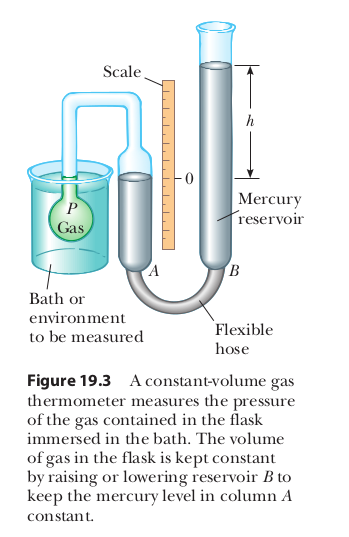
\includegraphics[scale=0.5]{temp_pres.png}
\end{center}


We can use this to find the linear relationship and the slope of the line. If we extrapolate the line to a pressure of 0, we see that the temperature will be around $-273.16$ degrees Celsius. This is true for different gases:


\begin{center}
	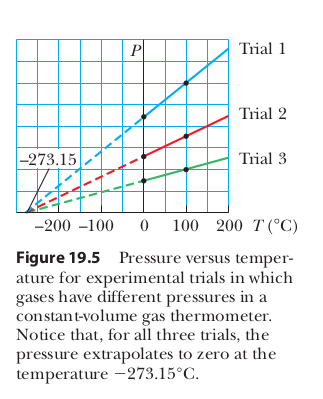
\includegraphics[scale=0.5]{temp_intepolate.png}
\end{center}


We can define a new scale based on this point. We define \textbf{absolute zero} where the temperature of a gas at constant pressure has an arbitrarily small pressure. We call this scale the \textbf{Kelvin scale}.

In addition, we made the value $273.16 K$ the triple point of water. This is so it would be easy to convert between this new absolute scale and the celsius scale:

$$T_K = T_C + 273.16 $$ 

In addition, there is the \textbf{Fahrenheit} scale used in the United States where the freezing point of water is $32$ and the boiling point is $212$

We know that the change in temperature from Fahrenheit will be the same as the change in temperature in Celsius, so:

$$(212-32)F = (100-0)C$$

$$1 C = \frac{9}{5}F$$

Thus one degrees Fahrenheit can be directly converted into Celsius and vice-versa.

Since we know that the freezing point of water is 0 degrees Celsius and 32 degrees Fahrenheit:
$$T_C = \frac{9}{5}T_F + 32$$


\section{One-Dimensional Expansion}

When there is a transfer in energy due to heat into an object, it usually expands.

Microscopically, at room temperature, molecules oscillate around their equilibrium point around $10^{-11} m$ and with a frequency of $10^{13}$ Hz. The spacing is around $10^{-10}$ m (so the spacing is smaller than the actual amplitude). Since when we heat the molecules the amplitude increases, usually creating a greater spacing in between them. 

If the expansion is small relative to the initial length, we can approximate the change in length as proportional to the change in temperature.

Thus:

$$
\boxed{
\Delta L = \alpha L_i \Delta T
}
$$

$$L_f = (1+\alpha\Delta T)L_i$$

Note that for some materials, $\alpha$ may be small for some dimensions because of the chemical structure of that material.


\section{Volumetric Expansion}
Let's assume we have a material that is \textbf{isotropic}, that is the coefficient of linear expansion is the same in all dimensions.

Let's consider a box with initial dimensions $l_i, w_i, h_i$. Since, we expect expansion in all dimensions:

$$l_f = (1+\alpha\Delta T)l_i$$
$$w_f = (1+\alpha\Delta T)w_i$$
$$h_f = (1+\alpha\Delta T)h_i$$


We know that the initial volume is $V = lwh$. Therefore, the new volume is:

$$V_f = l_fw_fh_f$$ 
$$= [(1+\alpha\Delta T)l_i][(1+\alpha\Delta T)w_i][](1+\alpha\Delta T)h_i]$$ 
$$= (1+\alpha\Delta T)^3l_iw_ih_i$$
$$V_f = (1+\alpha\Delta T)^3V_i$$

We know from the binomial theorem, that we can expand the cubic term out to:

$$V_f =  [1+3\alpha\Delta T + 3(\alpha\Delta T)^2 + (\alpha\Delta T)^3]V_i$$

The value of $\alpha$ is usually really small (on the order of $10^{-5}$). Thus, when we square and cube it, it will almost equal 0:

$$V_f \approx  (1+3\alpha\Delta T)V_i$$

This looks awfully lot like our expansion in one dimension formula.If we define:

$$\beta = 3\alpha$$

as our coefficient of volumetric expansion, we get:

$$V_f \approx  (1+\beta\Delta T)V_i$$

\section{Volumetric Expansion of Gases}








\chapter{First Law of Thermodynamics}
\section{Work and Heat}
Let us consider a system $S_\text{sys}$ and its surroundings $S_\text{surr}$.

We know that the net transfer of energy of a system is just the sum of individual transfers of energy (through work, matter, radiation, etc.). Let us consider the specific case where the only transfers of energy in and out of our system are work and heat.

Thus, from the principle of energy conservation:

$$
\boxed{
\Delta E = Q + W}
$$

where $Q$ is the heat transferred \textbf{to} the system and $W$ is the work done \textbf{on} the system. Notice that in this case, we are considering the work done on the system. Many textbooks use work done \textbf{by} the system on the surroundings instead and have $\Delta E = Q - W_{done}$. We will \textbf{not} be using this approach.

The first law of thermodynamics is simply just what we described above. It just says that the change in energy of a system is just the sum of the contribution from heat from the environment and the contribution of work from the environment.

\begin{mytheo}{First Law of Thermodynamics}{first_law}
    The change in the internal energy of a system is just the sum of the changes due to a transfer of heat energy from the environment to the system and a transfer of work from the environment to the system.
    
    $$\Delta E = Q + W$$

\end{mytheo}


Thus, it is possible to increase the total amount of energy of a system even while energy leaves the system through heat. All we need to do is provide enough energy from the environment through work.  

\section{Specific and Latent Heat}
We know from experience that when you heat something up, the temperature will rise. This is because transferring heat energy increases the internal energy of a system (provided that not much of it escapes due to work). Since the internal energy is directly related to the temperature, the temperature will rise as well (we will discuss this in far more detail later).

Let's first consider the case of a temperature change of a body (solid, liquid or gas) with mass $m$ away from the boiling/condensation and freezing/melting points. It turns out that in this case, the change in temperature is directly proportional to the heat put into the system and inversely proportional to the mass of the body. This should make intuitive sense, it is harder to change the temperature of a more massive body with the same amount of heat. It is also easier to make the temperature of a body increase with access to more heat energy.

We then have:

$$\Delta T \propto \frac{Q}{m}$$

Rearranging and introducing a proportionality constant $c$, we have:

$$Q = mc\Delta T $$

The value $c$ is called \textbf{specific heat}. It is different for different materials and at different temperatures. For example, $c$ is $4.186 \, J/K\cdot g$ at 4 degrees Celsius.


When a body is changing its state (from solid to liquid for example), something different occurs. Let's consider the case of water turning into steam for example, If we put heat into our system at, for example, 95 degrees Celsius and we watched the water warm up to 100 degrees Celsius, we will notice something peculiar happening. The water will stay at around 100 degrees Celsius (until all of the water is converted to steam) for some time even though we are applying significant amounts of heat energy to the system.

What is happening? It turns out that the energy we are providing is used to break the inter molecular bonds present in water to turn it into steam. Thus, the energy required to turn all of water into steam is directly proportional to the number of molecules or the mass of the body we are considering.

Thus, the magnitude of heat required to induce a state change in some body is only directly proportional to mass:

$$Q_L \propto m$$

$$Q_L = mc_L$$


The constant $c_L$ is called the \textbf{latent specific heat} and is dependent on the state change (solid - > liquid or liquid - > gas) and the properties of the body we're considering. It turns out that the heat required to break the bonds of a material is equal to the amount of heat given out when bonds begin to form again. For example, the amount of heat it takes to vaporize water is the same as the amount of heat that is released when it is condensing.

The figure below shows how adding energy to a system impacts temperature and where latent heat comes in:

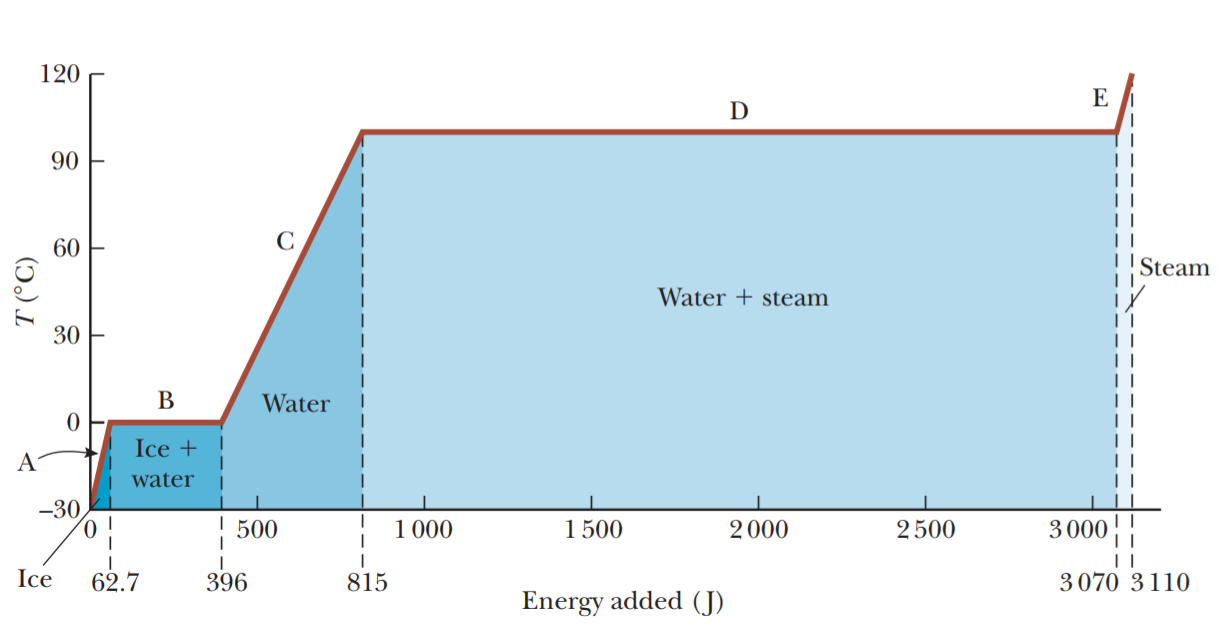
\includegraphics[scale=0.5]{energy_temp.PNG}




\section{Work and PV Diagrams}
In our analysis of analyzing systems through heat and work, it is often convenient to work with ideal gases. 

The reason we work with ideal gases is because it is often fairly easy to calculate the amount of work done by analyzing their pressure and volume.

Consider a gas in a cylinder with a mass-less friction-less piston on the top and some pressure $P_i$ from the environment. Furthermore, say that our system is in equilibrium such that the pressure from our gas is the same as the surroundings $P_i$. 

Let's say that we heat up the gas molecules inside such that the pressure inside is now $P_f > P_i$ causing it to expand and to do work (since we are applying a force over a distance). What is the work done by the expanding piston?

Let's call the surface area of the piston $A$ and the change in height of the piston $h$. The work done \textbf{by} the gas is:

$$W_{\text{by}} = \int{\mathbf{F} \cdot \dd \mathbf{h}} = \int{\mathbf{P_f}A \cdot \dd \mathbf{h}} $$

Since the force being applied is in the same direction of expansion:

$$\mathbf{P_f}A \cdot \dd \mathbf{h} =P_f A\dd h $$

We know that a small change in height times the surface area is just a small change in volume:

$$\dd V = A \dd h$$

Putting this together, we have the work done by the gas is:

$$W_{\text{by}} = \int_{V_i}^{V_f} P \dd V$$

We can do a similar derivation when we calculate the work by the gas when the volume contracts and get the same result.

For our discussion of thermodynamics, we want to consider the work done \textbf{on} the gas which is just the negative of the expression we got above:

$$\boxed{
W = -\int_{V_i}^{V_f} P \dd V
}$$

Thus, when the gas expands in a container against a piston in \textit{does} work and therefore work leaves our system and should be negative. When it contracts, something is doing work on the system and the work done on our system should be positive.

This leads us to an important visualization of thermodynamics through something we call \textbf{PV diagrams}. PV diagrams are diagrams where volume is graphed on the x axis and pressure is graphed in the y axis. 

We often want to consider processes that starts at some initial pressure $P_i$ and some initial volume $V_i$ and ends at another pressure and volume $P_f$ and $V_f$ with defined values for pressure and volume throughout the process. Since we found out that the absolute value of the work done on an ideal gas is just the integral of pressure over some volume difference, we know from calculus that this is just the area under the curve.

\begin{center}
    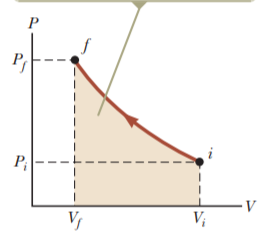
\includegraphics[scale=0.9]{pv_work.PNG}
\end{center}

Thus,

\begin{mytheo}{Work done by an Ideal Gas}{work_ideal}
    The work done  on an ideal gas expanding or contracting is:
    $$W = -\int_{V_i}^{V_f} P \dd V$$
    
    where $P$ is a function of $V$ giving us the pressure of the gas
    
    Therefore, we can calculate the magnitude of the work done by some process easily by just considering the area under the curve of a pressure-volume diagram.
    
    (The following is only true if the pressure and volume have a defined value throughout the expansion or contraction. Therefore, as we will discuss, adiabatic free expansion is an example where we can't just find the "area under the curve" since there is no curve to begin with).
    
\end{mytheo}




\section{Methods of Heat Transfer}
There are three main ways to transfer heat from one body to another. We will only briefly note them.

\subsection{Conduction}

Conduction occurs when you put a body at a higher temperature directly in contact with another body at a lower temperature. Heat will travel from the hotter object to the colder object.

Microscopically, since the hotter object has molecules with higher average translational kinetic energy, they will impart momentum on the colder body. Then the molecules in the colder body will also begin to start to move faster and push neighboring molecules. This process will continue until both bodies are at some equilibrium temperature.

We can quantify this is as well! Let's consider a rod of some material with one side hotter (at temperature $T_H$) and the other side cooler (at temperature $T_C$). Let's consider the rate at which heat transfers from one end to the other.

Heat will transfer faster if the temperature difference is greater and if the cross sectional area is greater (since there will be greater chances to impart momentum at each cross section). The rate at which heat transfers will also be inversely proportional to the length of the rod, since it will take longer to transfer the same amount of heat. Thus:

$$\frac{\Delta Q}{\Delta t} = -A\frac{\Delta T}{\Delta x}$$

or


$$\boxed{\dv{Q}{t} = -kA\dv{T}{x}}$$

where $k$ is the \textbf{thermal conductivity} and $\dv{T}{x}$ is the \textbf{temperature gradient} (how temperature varies over distances). The negative sign comes from heat transferring away from the hot body to the cold body (in the direction opposite to x)

For example, in the case where the left end of a rod is in contact with a \textbf{reservoir} at a temperature $T_C$ and the right end of the rod is in contact with another reservoir at temperature $T_H$, the temperature gradient between the two rods should be constant:
\begin{center}
    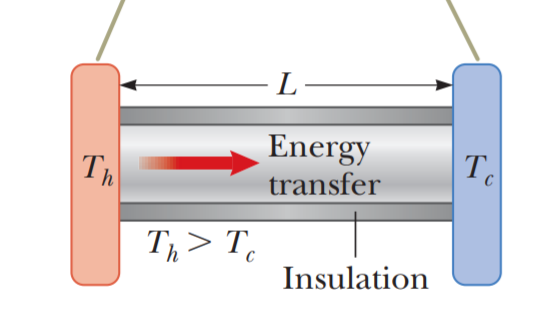
\includegraphics[scale=0.5]{conduction.PNG}
\end{center}

$$\dv{T}{x} = \frac{\Delta T}{\Delta x} = \frac{T_H-T_C}{L}$$

(This is true if no heat leaves the system and both sides of the rod are at the respective temperatures $T_H$ and $T_C$)

Thus, the rate at which heat transfers is:

$$\dv{Q}{t} = -kA\frac{T_H-T_C}{L}$$

When we have multiple rods connecting two reservoirs in parallel, we can directly add together the rates of energy transfer to get:


$$\dv{Q_{\text{tot}}}{t} = -\sum_i^N\dv{Q_i}{t} = -\sum_i^Nk_iA_i\frac{T_H-T_C}{L} = -\frac{T_H-T_C}{L}\sum_i^N k_iA_i$$

What about when we have two rods connecting two reservoirs in series in a steady state? This is a bit more complicated.

Let's consider the rate of heat transfer at the boundary of the rods. Let's say that the temperature there is $T$. We know that the rate of heat transfer from the left rod is:

$$\dv{Q}{t} = -k_1A\frac{T_H-T}{L_1} $$

We also know that the rate of heat temperature from the middle point to the end point is:

$$\dv{Q}{t} =- k_2A\frac{T-T_C}{L_2}$$

Since we're considering a steady state transfer of heat, these rates must be equal with each other:

$$-k_1A\frac{T_H-T}{L_1} = -k_2A\frac{T-T_C}{L_1}$$

Rearranging and solving for $T$, we get:

$$T = \frac{L_2k_1T_H+L_1k_2T_C}{L_2k_1+L_1k_2}$$

Putting this into one of our expressions above, we get:

$$\boxed{\dv{Q}{t} = -kA\frac{T_H-T_C}{(L_2/k_2+L_1/k_1)} }$$

We can expand this analysis even further by any number of materials connected in series:

$$\boxed{\dv{Q}{t} = -A\frac{T_H-T_C}{\sum_i^NL_i/k_i} }$$

\begin{center}
    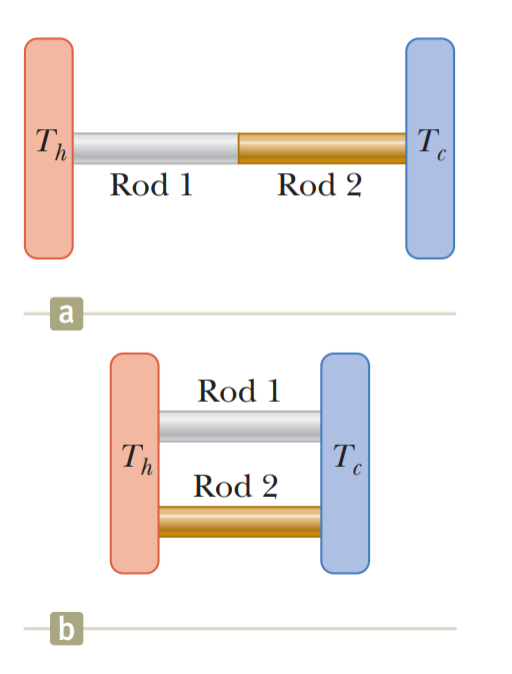
\includegraphics[scale=0.5]{con_series_par.PNG}
\end{center}

\subsection{Convection}

Convection is a form of matter transfer. It occurs when heat transfers from one system to another due to actual molecules with heat energy moving. Usually convection is a property of fluids becoming less dense as they have more heat energy, and thus moving in response to this.

The actual math of convection is quite complicated and will not be discussed in this section.

\subsection{Radiation}

All molecules produce radiation through electromagnetic waves from thermal vibrations. 

The rate at which an object radiates heat is given by \textbf{Stefan's Law}:

$$\boxed{P = \sigma AeT^4}$$

where $\sigma$ is a constant  $5.66963 \times 10^{-8}$ W/$m^2 \cdot K^4$, $A$ is the surface area, $e$ is the \textbf{emissivity} constant (equal to how much light something absorbs).

This is how we receive energy from the sun!

As an object radiates heat, it also absorbs it from the surroundings. Thus, the net amount of heat transferred is:

$$P = \sigma e(T^4-T_0^4)$$




\chapter{Kinetic Theory of Gases}
\section{Kinetic Model}

We are going to consider a simple model of ideal gases held in a square box with lengths $d$. In our model, the gas molecules will be extremely small point masses that never collide with one another and are bouncing off the walls like in the figure shown below.

\begin{center}
    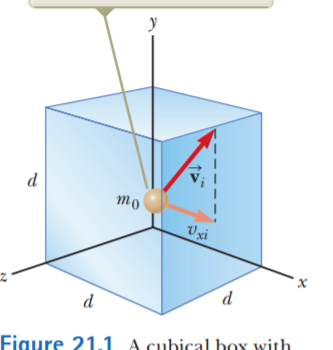
\includegraphics[scale=0.5]{kinetic_model.PNG}
\end{center}

Let's first consider one gas molecule with mass $m$ and a velocity in the x direction $v_x$. Let's consider the collision of the gas molecule with a wall.

\begin{center}
    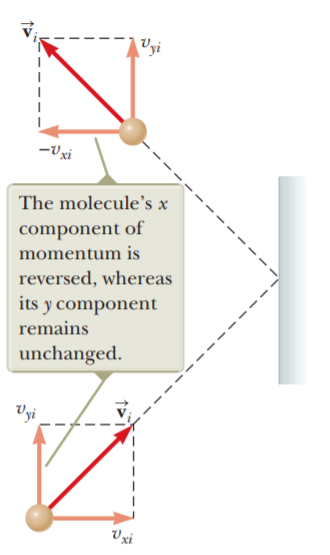
\includegraphics[scale=0.5]{kin_mod_bounce.PNG}
\end{center}
Because of the principles of conservation of kinetic energy, the magnitude of the velocity before and after the collision should be the same. 

We also know that the momentum of the gas molecule has changed from $mv_x$ to $-mv_x$. This means that the wall must have applied an impulse of $-2mv_x$:

$$\int F_{w}\dd t = -2mv_x$$

From Newton's Third Law, we know that the force exerted by the wall on the molecule must be the equal and opposite as the force from the molecule onto the wall, so the impulse from the gas molecule is:

 
$$\int F_{g}\dd t = 2mv_x$$


The molecule will then travel to the other end of the box, bounce back and hit the wall again after some time in our simple model. Therefore the force with respect to time will look something like this:


We can calculate the average force on the wall by the gas molecule:

$$\int F_{g}\dd t = \overline{F_g}\Delta t = 2mv_x$$

$$\overline{F_g} = \frac{2mv_x}{\Delta t}$$

Note that this average force isn't really a force on the wall! It is just a continuous approximation of a discrete process. We can think about this as "flattening" out the jumps we had in the earlier figure. This will become useful when we have many gas molecules.

How can we find $\Delta T$, the time it takes for a molecule to collide back into the same wall? If the magnitude of the velocity is $v_x$ and the distance traveled is $2d$ (one $d$ while hitting the other wall and another $d$ while coming back). Using basic kinematics, we know that:

$$\Delta t = \frac{2d}{v_x}$$

Putting this into our expression, we have:

$$\overline{F_g} = \frac{mv_x^2}{d}$$

Now, we know that a gas is composed of many molecules (on the order of $10^{23}$). In order to find the average force on one wall, we can sum up the average force of each gas molecule:

$$\overline{F_{tot}} = \sum_i^N\overline{F_{g,i}} = \frac{m}{d}\sum_i^Nv_{i,x}^2$$

Let's consider the average of the squared velocities of these gas molecules.

$$\overline{v_x^2} = \frac{1}{N}\sum_i^Nv_{i,x}^2 $$

$$\sum_i^Nv_{i,x}^2  = N\overline{v_x^2}$$

Subbing this into our expression, we get that:

 
$$\overline{F_{tot}} = \frac{Nm\overline{v_x^2}}{d}$$


Since we're considering an enormous number of gas molecules, the average force on the wall by the molecules approaches the actual force on the wall.

$$\boxed{F_{tot} = \frac{Nm\overline{v_x^2}}{d}}$$

Through this entire process, we've been considering molecules moving in all three dimensions. Thus, from Pythagoras Theorem, we know that:

$$\sum_i^N v_i^2 = \sum_i^N v_{i,x}^2  + \sum_i^N v_{i,y}^2 + \sum_i^N v_{i,z}^2$$ 

$$N\overline{v^2} = N\overline{v_x^2} + N\overline{v_y^2}+N\overline{v_z^2}$$

If we assume that $$\overline{v_x^2} \approx \overline{v_y^2} \approx \overline{v_z^2}$$,

$$\overline{v^2} \approx 3\overline{v_x^2}$$

$$\overline{v_x^2} = \frac{1}{3}\overline{v^2}$$

where $\overline{v^2}$ through this entire process is the average of the magnitude of squared velocities of each molecule. 

Putting this into our expression, we get:
$$F_{tot} = \frac{Nm\overline{v^2}}{3d}$$

We know the area of the wall that the gas molecules are hitting is $d^2$. Thus,

$$Pd^2 = \frac{Nm\overline{v^2}}{3d}$$

$$Pd^3 = \frac{Nm\overline{v^2}}{3}$$

Since $V = d^3$, this gives us:

$$\boxed{PV = \frac{Nm\overline{v^2}}{3}}$$

Using the ideal gas law, we know that $PV = Nk_bT$ (an experimental result). Putting this into our equation, we get that:

$$PV = Nk_bT = \frac{Nm\overline{v^2}}{3}$$

$$k_bT = \frac{2}{3} (\frac{1}{2}m\overline{v^2})$$

$$\boxed{K_{trans, avg} = \frac{1}{2}m\overline{v^2} = \frac{3}{2}k_bT}$$


which is a beautiful result! The formula above shows us that the temperature is directly proportional to the average translational kinetic energy. This justifies the definition of temperature we described early in these notes.

\section{Thermodynamic Processes}




\chapter{Heat Engines and Entropy}
\section{Second Law of Thermodynamics}
\section{Reversibility}
\section{Carnot Cycle}











\chapter{Questions}
\begin{itemize}
    \item From a microscopic level, why does a hole grow during thermal expansion?
    
    \item Is any process we can draw on a PV diagram possible to be replicated as a reversible process?
    \item Is the efficiency of any reversible engine the same as the Carnot Cycle?
    \item Given a reversible Stirling cycle (adiabatic + iso-volumetric process), how does the efficiency compare to that of the Carnot engine. 
    
    
    
    \item What is entropy? Is the entropy of a macrostate the amount of uncertainty we have for any particular microstate?
    \item It the entropy of any reversible cycle equal to 0?
    \item Why does entropy increase with respect to time.
    \item Is the following formular correct for calculating a change in entropy:
    
    $$\Delta S = Nk_B\left[\frac{f}{2}\ln(T_f/T_i) + \ln(V_f/V_i)\right]$$
    
    where $f$ is the number of degrees of freedom for an ideal gas
    
    \item Can we talk about the entropy of something like we can with energy. Or is the primary definition in terms of $\Delta S$ and we can set an arbritrary 0 point like we did with energy?
    \item 
    
    
    
\end{itemize}

\newpage



\end{document}
